\documentclass[]{article}
\usepackage{amsmath}
\usepackage{geometry}
\geometry{legalpaper, portrait, margin=1in}
\usepackage{algorithm}
\usepackage{algorithmic}
\usepackage{tikz}

%opening
\title{Exploring a Non-Parametric Bayesian Perspective\\ on Compositional Contextual Inference in Motor Learning}
\author{Daniel Kornai}

\begin{document}

\maketitle


\section{Formulating The Problem}
Visual stimulus will impact motor learning if the learner believes that visual and motor signals share a common latent cause. This common latent cause [sometimes called \textit{context}] may be used to index visuo-motor experiences in a way that permits compact and generalisable representations.

In a series of trials of a motor learning experiment, we observe a $D$ dimensional force vector $\mathbf{f}$, and a $T$ dimensional binary visual cue $\mathbf{x}$ a total of $N$ times. If we believe these observations were caused by a latent variable that simultaneously controls both types of sensory experience, then the $N \times D$ matrix $\mathbf{F}$ and the $N \times T$ matrix $\mathbf{X}$ can be factored into a pair of basis sets [$\mathbf{A}$ and $\mathbf{Y}$ for forces and visuals respectively] and a shared binary feature ownership matrix $\mathbf{Z}$. That is, the $i$-th row of $\mathbf{A}$ and $\mathbf{Y}$ together form a prototypical visuo-motor sensory context, which we believe is contributing to our observations in the $n$-th trial if $\mathbf{Z}_{n,i} = 1$. Additional expressive richness [and compressive capability] is conferred on such a factorisation model if multiple contexts can be \textit{composed} with each other.

In this setup we are essentially searching for the solutions to the matrix equations $\mathbf{X} \approx \mathbf{Z}\mathbf{Y}$ and $\mathbf{F} \approx \mathbf{Z}\mathbf{A}$, which nicely corresponds to finding the posterior distributions of $\mathbf{Z}$, $\mathbf{Y}$, and $\mathbf{A}$ given our data $\mathbf{X}$, $\mathbf{F}$, and contraints given by the priors on our unknowns. From Bayes rule, 
\begin{equation}
	P(\mathbf{Z}, \mathbf{Y}, \mathbf{A} | \mathbf{X}, \mathbf{F}) \propto P(\mathbf{Z})P(\mathbf{X}|\mathbf{Z}, \mathbf{Y})P(\mathbf{Y})p(\mathbf{F}|\mathbf{Z},\mathbf{A})p(\mathbf{A})
\end{equation}
where we assumed the independence structure shown in the graphical model of Fig. \ref{fig:graphmod}, which we will detail later. The formulation of this problem as Bayesian inference expresses our desire to find representations that generates observations with high probability [as captured by the likelihoods], and finding a representations that are in general probable, as expressed by the priors. 
\begin{figure}[H]\label{fig:graphmod}
	\begin{center}
		\scalebox{0.8}{
		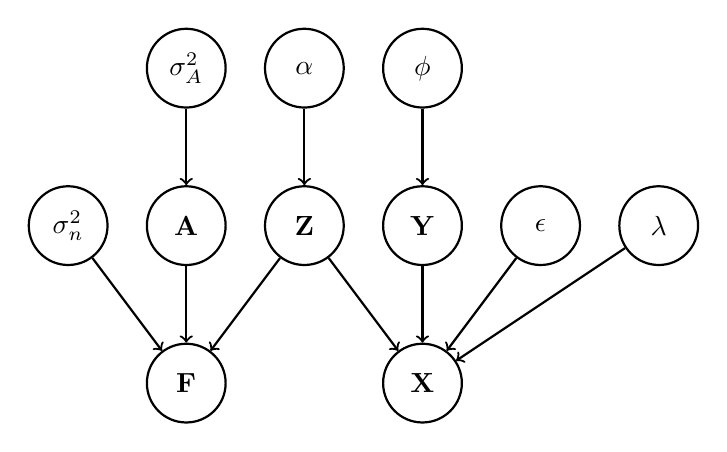
\begin{tikzpicture}[node distance=1.5cm and 2cm, 
			every node/.style={draw, circle, minimum size=1cm, inner sep=0pt}, 
			every path/.style={->, thick}]
			
			% Define the nodes for the first line
			\node (A1) at (-1.5, 4) {$\sigma^2_A$};
			\node (A2) at (0, 4) {$\alpha$};
			\node (A3) at (1.5, 4) {$\phi$};
			
			% Define the nodes for the second line
			\node (B1) at(-3, 2) {$\sigma^2_n$};
			\node (B2) at(-1.5, 2) {$\mathbf{A}$};
			\node (B3) at(0, 2) {$\mathbf{Z}$};
			\node (B4) at(1.5, 2) {$\mathbf{Y}$};
			\node (B5)  at(3, 2) {$\epsilon$};
			\node (B6)  at(4.5, 2) {$\lambda$};
			
			% Define the nodes for the third line
			\node (C1) at (-1.5, 0){$\mathbf{F}$};
			\node (C2)at (1.5, 0){$\mathbf{X}$};
			
			% Optional: Draw lines or customize positioning
			\draw (A1) -- (B2);
			\draw (A2) -- (B3);
			\draw (A3) -- (B4);
			\draw (B1) -- (C1);
			\draw (B2) -- (C1);
			\draw (B3) -- (C1);
			\draw (B3) -- (C2);
			\draw (B4) -- (C2);
			\draw (B5) -- (C2);
			\draw (B6) -- (C2);
		\end{tikzpicture}
		}
	\end{center}
	\caption{Graphical model illustrating dependencies among variables in the generative model.}
\end{figure}	

Our prior expectation is that rows of $\mathbf{A}$ are drawn from $\mathcal{N}(0, \sigma^2_A \mathbf{I})$. Forces are assumed to be observed under a linear Gaussian model where the hyperparameter $\sigma^2_n$ controls the magnitude of observation noise. 
\begin{equation*}
	f_{n,:} = \mathbf{x}_{n,:}\mathbf{A} + \epsilon \sim \mathcal{N}(0, \sigma^2_n, \mathbf{I})
\end{equation*}

Each element of $\mathbf{Y}$ is drawn independently as $y_{i,k} \sim \text{Bernoulli}(\phi)$. The entries of $\mathbf{X}$ are conditionally independent given the latents, and are assumed to be generated from a \textit{noisy-OR} distribution
\begin{equation}
	P(x_{i,t} = 1 | \mathbf{Z}, \mathbf{Y}) = 1 - (1-\lambda)^{\mathbf{z}_{i,:}\mathbf{y}_{:,t}}(1-\epsilon)
\end{equation}
where $\mathbf{z}_{i,:}\mathbf{y}_{:,t} = \sum_{k=1}^{K} \mathbf{z}_{i,k}\mathbf{y}_{k,t}$ is the number of latent causes that have the $t$-th pixel as 1. $\epsilon$ is the baseline probability that $x_{i,t} = 1$, and $\lambda$ is the probability with which any of the hidden causes is effective in eliciting a visual signal. 

While the number of rows for $\mathbf{Z}$ is fixed by the number of observations, the number of distinct visuo-motor contexts ($K$) required to effectively represent the set of experiences during the trial depend on the statistics of the data and the beliefs of the observer. To account for this, our prior distribution on $\mathbf{Z}$ utilises the Indian Buffet Process [IBP]. This allows us to sample from a distribution of sparse binary matrices with a fixed number of rows and a potentially infinite number of columns. The hyperparameter $\alpha$ controls our propensity to add new features (columns of $\mathbf{Z}$) during the learning process.

Given a dataset, we utilise a Gibbs sampler to collect samples from $\mathbf{Z}$, $\mathbf{Y}$, and $\mathbf{A}$. Details of this sampling procedure, which iteratively grows the number of latent features, are provided below:

\newpage
\section{Algorithm for Gibbs Sampler}
An outline of the sampling procedure is:

\begin{algorithm}[H]
	\caption{Outline for the Gibbs sampler $P(\mathbf{Z}, \mathbf{Y}, \mathbf{A} | \mathbf{X}, \mathbf{F})$}
	\begin{algorithmic}[1]
		\REQUIRE Force observations $\mathbf{F}$, Visual observations $\mathbf{X}$, initial number of features $K$.
		\vspace{0.2cm}
		
		\STATE initialise $\mathbf{Z}$, $\mathbf{A}$ and $\mathbf{Y}$.
		\vspace{0.2cm}
		
		\WHILE{gathering posterior samples}
		\vspace{0.2cm}
		
		\STATE resample $\mathbf{A}$ \\
		\vspace{0.2cm}
		
		\STATE resample $\mathbf{Y}$ \\
		\vspace{0.2cm}
		
		\FOR{$i = 1$ to $N$}
		\vspace{0.2cm}
			\STATE resample $\mathbf{Z}$
			\vspace{0.2cm}
		
			\STATE sample the number of new features $K^{new}_i$
			\vspace{0.2cm}
		
			\IF{$K^{new}_i > 0$}
				\STATE expand $\mathbf{Z}$, $\mathbf{A}$, $\mathbf{Y}$
				
			\ENDIF
		\vspace{0.2cm}
		
		\ENDFOR
		
		\ENDWHILE
	\end{algorithmic}
	\label{alg:gs}
\end{algorithm}

The complete algorithm is

\begin{algorithm}[H]
	
	\caption{Gibbs sampler for $P(\mathbf{Z}, \mathbf{Y}, \mathbf{A} | \mathbf{X}, \mathbf{F})$}
	\begin{algorithmic}[1]
		\REQUIRE Force observations $\mathbf{F}$, Visual observations $\mathbf{X}$, initial number of features $K$.
		\vspace{0.2cm}
		
		\STATE $ \mathbf{Z} \gets P(\mathbf{Z})$ \hfill \COMMENT{Initialise $N \times K$ feature ownership matrix $\mathbf{Z}$ from the prior}
		\STATE $ \mathbf{A} \gets P(\mathbf{A})$ \hfill \COMMENT{Initialise $K \times D$ force basis matrix $\mathbf{A}$ from the prior}
		\STATE $ \mathbf{Y} \gets P(\mathbf{Y})$ \hfill \COMMENT{Initialise $K \times T$ image filter basis matrix $\mathbf{Y}$ from the prior}
		\vspace{0.2cm}
		
		\WHILE{gathering posterior samples}
		\vspace{0.2cm}
		
			\STATE $\mathbf{A} \gets p(\mathbf{A}|\mathbf{F}, \mathbf{Z})$ \hfill \COMMENT{Resample $\mathbf{A}$ according to Eq. \ref{eq:posterior_A}}
			\vspace{0.2cm}
			
			\FORALL{$y_{k,t} \in \mathbf{Y}$}
				\STATE $y_{k,t} \gets P(y_{kt}|\mathbf{Z}, \mathbf{X}, \mathbf{Y}_{-k,t})$ \hfill \COMMENT {Resample each element of $\mathbf{Y}$ according to Eq. \ref{eq:posterior_Ykt}}
			\ENDFOR
			\vspace{0.2cm}
			
			\FOR{$i = 1$ to $N$}
				\vspace{0.2cm}
				\FOR{$k = 1$ to $K$} 
					\STATE $m_{-i,k} \gets \sum_{j\not=k}^{N}z_{j,k}$ \hfill \COMMENT{Count objects that own feature $k$ without considering object $i$}
					\IF{$m_{-i,k} > 0$}
						\STATE $z_{i,k} \gets P(z_{i,k}|\mathbf{f}_{i,:}, \mathbf{x}_{i,:}, \mathbf{A}, \mathbf{Y}, \mathbf{Z}_{-i,k})$ \hfill \COMMENT{Resample $z_{i,k}$ according to Eq. \ref{eq:posterior_Zik}}
					\ELSE
						\STATE mark $z_{i,k}$ to be zeroed
					\ENDIF
				\ENDFOR
				\STATE set all marked $z_{i,k}$ to $0$ 
				\vspace{0.2cm}
				
				\STATE $K^{new}_i \gets P(K^{new}_i | \mathbf{x}_{i,:},  \mathbf{f}_{i,:}, \mathbf{z}_{i,: }, \mathbf{Y}, \mathbf{A})$ \hfill \COMMENT{Sample $K^{new}_i $ according to Eq. \ref{eq:posterior_Knew}}
				\vspace{0.2cm}

				
				\IF{$K^{new}_i > 0$}
					\STATE $\mathbf{Z}_{new} \gets Z_{new}[K^{new}_i , i]$ \hfill  \COMMENT{Get $K^{new}_i $ new columns for $\mathbf{Z}$, each with a $1$ at row $i$}
					\STATE  $\mathbf{A}_{new} \gets p(\mathbf{A}_{new}| \mathbf{F}, \mathbf{Z}_{new}, \mathbf{Z}, \mathbf{A})$ \hfill \COMMENT{Get $K^{new}_i $ new rows for $\mathbf{A}$, sampled from Eq. \ref{eq:posterior_Anew}}
					\STATE $\mathbf{Z} \gets [ \mathbf{Z}, \mathbf{Z}_{new}]$\hfill \COMMENT{Expand $\mathbf{Z}$ with the new columns}
					\STATE $\mathbf{A} \gets [ \mathbf{A}; \mathbf{A}_{new}]$ \hfill \COMMENT{Expand $\mathbf{A}$ with the new rows}
					\STATE $\mathbf{Y}_{new} \gets 0_{k^{new}_i  \times T} $  \hfill \COMMENT{Get $K^{new}_i $ new empty rows for $\mathbf{Y}$}
					\STATE $\mathbf{Y} \gets [ \mathbf{Y}; \mathbf{Y}_{new}]$ \hfill \COMMENT{Expand $\mathbf{Y}$ with the new rows}
					\FORALL{$y_{k,t} \in \mathbf{Y}_{K+1:K+K{new}_i},:$}
						\STATE $y_{k,t} \gets P(y_{kt}|\mathbf{Z}, \mathbf{X}, \mathbf{Y}_{-k,t})$ \hfill \COMMENT {Resample the new parts of $\mathbf{Y}$ according to Eq. \ref{eq:posterior_Ykt}}
					\ENDFOR
					\STATE $K \gets K + K^{new}_i$ 
				\ENDIF
				\vspace{0.2cm}
				
			\ENDFOR

		\ENDWHILE
	\end{algorithmic}
	\label{alg:gso}
\end{algorithm}


\newpage
\section{Posterior Terms Used During Sampling}

\subsection{Posterior $p(\mathbf{A}|\mathbf{F}, \mathbf{Z})$}
Given the observed forces $\mathbf{F}$, and the binary feature ownership matrix $\mathbf{Z}$, the posterior $\mathbf{A}$ is sampled from from the following Gaussian 
	\begin{equation}\label{eq:posterior_A}
		p(\mathbf{A}|\mathbf{F}, \mathbf{Z}) \sim \mathcal{N}\left( \left(\mathbf{Z}^T \mathbf{Z} + \frac{\sigma^2_n}{\sigma^2_A}\mathbf{I}\right)^{-1} \mathbf{Z}^T \mathbf{F} , \sigma^2_n \left(\mathbf{Z}^T \mathbf{Z} + \frac{\sigma^2_n}{\sigma^2_A}\mathbf{I}\right)^{-1}  \right)
	\end{equation}


\subsection{Posterior $P(y_{k,t}|\mathbf{Z}, \mathbf{X}, \mathbf{Y}_{-k,t})$}
When performing updates to $\mathbf{y}_{:,t}$, the $t$-th column of the image filter basis matrix $\mathbf{Y}$, this impacts the $t$-th column of the reconstructed images. Accordingly, the posterior from proportional is
\begin{align}
	\begin{split}\label{eq:posterior_Ykt}
		&P(y_{k,t}=a|\mathbf{Z}, \mathbf{X}, \mathbf{Y}_{-k,t}) \\
		&\quad \propto P(y_{k,t}=a) P(\mathbf{x}_{:,t}|\mathbf{Z}, \mathbf{y}_{:,t})|_{y_{k,t}=a} \\
	\end{split}
\end{align}

The prior is defined using the hyperparameter $\phi$ as 
\begin{align}
	P(y_{k,t}=a) = \phi^a (1-\phi)^{1-a}
\end{align}

And the likelihood is:
\begin{align}
	\begin{split}\label{eq:lik_pxt}
		&P(\mathbf{x}_{:,t}|\mathbf{Z}, \mathbf{y}_{:,t}) =\prod_{i=1}^{N} \left[1 - (1-\lambda)^{\mathbf{z}_{i,:}\mathbf{y}_{:,t}}(1-\epsilon)\right]^{x_{i,t}} \times \left[ (1-\lambda)^{\mathbf{z}_{i,:}\mathbf{y}_{:,t}}(1-\epsilon)\right]^{1 - x_{i,t}} 
	\end{split}
\end{align}

 $|_{y_{k,t}=a}$ denotes carrying out the calculation with $y_{k,t}$ temporarily set to $a$.

\subsection{Posterior $P(z_{i,k}|\mathbf{f}_{i,:}, \mathbf{x}_{i,:}, \mathbf{A}, \mathbf{Y}, \mathbf{Z}_{-i,k})$}
As our force and image observations are conditionally independent given $\mathbf{Z}$, our posterior proportional is
	\begin{align}
		\begin{split}\label{eq:posterior_Zik}
			&P(z_{i,k}=a|\mathbf{f}_{i,:}, \mathbf{x}_{i,:}, \mathbf{A}, \mathbf{Y}, \mathbf{Z}_{-i,k}) \\
			&\quad \propto P(z_{i,k}=a| \mathbf{Z}_{-i,k}) P(\mathbf{x}_{i,:}|\mathbf{Y}, \mathbf{z}_{i,:})  p(\mathbf{f}_{i,:}|\mathbf{A}, \mathbf{z}_{i,:})|_{z_{i,k}=a} 
		\end{split}
	\end{align}

The prior $P(z_{i,k}=a| \mathbf{Z}_{-i,k})$ is defined with $m_{-i,k} = \sum_{j\not=i}^{N} z_{j,k}$ as
\begin{align}
	P(z_{i,k}=a| \mathbf{Z}_{-i,k}) = (\frac{m_{-i,k}}{N})^a (1 - \frac{m_{-i,k}}{N})^{1-a}
\end{align}


The likelihood term for the visual observation is $P(\mathbf{x}_{i,:}|\mathbf{Y}, \mathbf{z}_{i,:})$ is 
\begin{align}
	&P(\mathbf{x}_{i,:}|\mathbf{Y}, \mathbf{z}_{i,:}) = \prod_{t=1}^{T} \left[1 - (1-\lambda)^{\mathbf{z}_{i,:}\mathbf{y}_{:,t}}(1-\epsilon)\right]^{x_{i,t}} \times \left[ (1-\lambda)^{\mathbf{z}_{i,:}\mathbf{y}_{:,t}}(1-\epsilon)\right]^{1 - x_{i,t}} 
\end{align}

\noindent and the likelihood term for the force observation is $p(\mathbf{f}_{i,:}|\mathbf{A}, \mathbf{z}_{i,:})$ is simply
\begin{align}
	&p(\mathbf{f}_{i,:}|\mathbf{A}, \mathbf{z}_{i,:}) = \frac{1}{(2\pi\sigma^2_n)^{D/2}} \exp \left(-\frac{1}{2\sigma^2_n} (\mathbf{f}_{i,:} - \mathbf{z}_{i,:} \mathbf{A})^T (\mathbf{f}_{i,:} - \mathbf{z}_{i,:} \mathbf{A}) \right)
\end{align}

As previously, The symbol $|_{z_{i,k}=a}$ denotes carrying out the calculation with $z_{i,k}$ temporarily set to $a$.

\subsection{Posterior $P(K^{new}_i | \mathbf{x}_{i,:},  \mathbf{f}_{i,:}, \mathbf{z}_{i,: }, \mathbf{Y}, \mathbf{A}) $}
During the process of sampling, it might be necessary to increase the number of latent features. As new features is initially only active for the $i$-th row of $\mathbf{z}$
	\begin{align}
		\begin{split}\label{eq:posterior_Knew}
		&P(K^{new}_i | \mathbf{x}_{i,:},  \mathbf{f}_{i,:}, \mathbf{z}_{i,: }, \mathbf{Y}, \mathbf{A}) \\
		&\quad \propto P(k^{new}_i) P(\mathbf{x}_{i,:}| \mathbf{z}_{i,:}, \mathbf{Y}, K^{new}_i) p(\mathbf{f}_{i,:}|\mathbf{z}_{i,:}, \mathbf{A}, K^{new}_i)
	\end{split}
	\end{align}

The prior $P(k^{new}_i)$ is simply a Poisson:
\begin{align}
	P(k^{new}_i) = \text{Pois}\left(\frac{\alpha}{N}\right)
\end{align}
	
The likelihood term for the visual observations given $K^{new}_i$ is
	\begin{align}
		\begin{split}
			&P(\mathbf{x}_{i,:}| \mathbf{z}_{i,:}, \mathbf{Y}, K^{new}_i) \\
			&\quad=  \prod_{t=1}^{T} \left[1 - (1-\epsilon)(1-\lambda)^{\mathbf{z}_{i,:}\mathbf{y}_{:,t}}(1-\lambda\phi)^{K^{new}_i}\right]^{x_{i,t}} \times \left[ (1-\epsilon)(1-\lambda)^{\mathbf{z}_{i,:}\mathbf{y}_{:,t}}(1-\lambda\phi)^{K^{new}_i}\right]^{1 - x_{i,t}} 
		\end{split}
	\end{align}
	
The likelihood for the force observations given $K^{new}_i$ is
 	\begin{align}
 		\begin{split}
 			&p(\mathbf{f}_{i,:}|\mathbf{z}_{i,:}, \mathbf{A}, K^{new}_i) = \int p(\mathbf{f}_{i,:}|\mathbf{z}_{i,:}, \mathbf{A}, \mathbf{A}_{new}, K^{new}_i)p(\mathbf{A}_{new}) \text{d} \mathbf{A}_{new} \\
 			&\quad= \frac{1}{[2 \pi (\sigma^2_n + K^{new}_i\sigma^2_a)]^{D/2}}	\exp \left(-\frac{1}{2(\sigma^2_n + K^{new}_i\sigma^2_a)} (\mathbf{f}_{i,:} - \mathbf{z}_{i,:} \mathbf{A})^T (\mathbf{f}_{i,:} - \mathbf{z}_{i,:} \mathbf{A}) \right)
 		\end{split}
 	\end{align}
Note how this reduces to the basic likelihood if  $K^{new}_i = 0$.
	
\subsection{Posterior $p(\mathbf{A}_{new}| \mathbf{F}, \mathbf{Z}_{new}, \mathbf{Z}, \mathbf{A})$}
	When $k_{new}$ features were added to $\mathbf{Z}$ in the form of $\mathbf{Z}_{new}$, $\mathbf{A}$ must also be expanded with $k_{new}$ rows. These rows are drawn from the following Gaussian
	\begin{align}
		\begin{split}\label{eq:posterior_Anew}
			&p(\mathbf{A}_{new}| \mathbf{F}, \mathbf{Z}_{new}, \mathbf{Z}, \mathbf{A}) \\
			&\quad \propto p(A_{new}) p(\mathbf{F} | \mathbf{Z}_{new}, \mathbf{Z}, \mathbf{A}, \mathbf{A}_{new}) \\
			&\quad \sim \mathcal{N}\left( \left(1_{k_{new}\times k_{new}}  + \frac{\sigma^2_n}{\sigma^2_A}\mathbf{I}\right)^{-1} \mathbf{Z}^T_{new} (\mathbf{F} - \mathbf{Z} \mathbf{A}), \sigma^2_n \left(1_{k_{new}\times k_{new}}  + \frac{\sigma^2_n}{\sigma^2_A}\mathbf{I}\right)^{-1}  \right)
		\end{split}
	\end{align}

\end{document}
